\section{Method}
\label{sec:method}

We study residual vision networks as a three-part map.
Stages~1--2 encode the image onto an input manifold; the longest stage
transports a point $x_0$ on that manifold to a point $x_T$ on an output manifold;
stage~4 and the prediction head decode $x_T$ into class logits.
We focus on that middle transport---stage~3 in ConvNeXt, Swin and ResNet---where
most of the residual depth sits.
In ConvNeXt-T, stage~3 has $n{=}9$ blocks; we take the trained horizon to be
$T{=}n{=}9$ and refine discretisations with repetitions $R$ and step
$\Delta t{=}1/R$ (\cref{sec:indefinite_looping}).

The question is whether this transport requires $n$ independent residual maps, or
whether it is (approximately) the integration of one vector field.
We organise the section accordingly:
\begin{enumerate}
    \item \cref{sec:weight_tied} shows that a weight-tied stage~3 nearly matches an
    untied ConvNeXt-T, so one shared field already carries most of the accuracy;
    \item \cref{sec:indefinite_looping} tests the Euler expansion over the residual blocks by
    looping them at inference without fine-tuning, on both weight-tied and standard
    networks;
    \item \cref{sec:geometrical_analysis} compares the geometry of the resulting
    trajectories (autonomous vs.\ switched fields);
    \item \cref{sec:overparametrized_undoing} examines how untied blocks redirect
    and partially undo each other along depth;
    \item \cref{sec:deltas} asks whether small per-block corrections on top of a
    shared field can close the remaining gap.
\end{enumerate}

\subsection{A weight-tied stage as an autonomous control}
\label{sec:weight_tied}

To separate what depends on having nine independent blocks from what depends only on
the residual form, we train a ConvNeXt-T whose stage~3 applies one shared block nine
times.
Reusing blocks of a model that was trained with distinct blocks tests a different
object, and fails (\cref{app:block-ops}); here the stage is \emph{trained} to use a
single function.
Both models are trained by us on ImageNet-1k for $300$ epochs with the same
augmentation, regularisation, optimiser and effective batch size of $1024$.
The runs are not matched in every setting: the untied model uses peak learning rate
$5{\times}10^{-4}$ with a $20$-epoch warmup on a single process, the tied one
$1{\times}10^{-3}$ with a $10$-epoch warmup on four distributed processes; no run
fixes a seed (\cref{app:training}).
The accuracy gap below is therefore indicative, not a controlled ablation.

The untied ConvNeXt-T reaches $80.96\%$ top-1 with $28.59$M parameters, below the
$82.1\%$ of the original recipe~\citep{liu2022convnext}, which uses a batch of $4096$.
The weight-tied model reaches $80.34\%$ with $18.97$M parameters ($33\%$ fewer,
$-0.62$ points), and sharing one block per stage in all four stages reaches $78.99\%$
with $8.68$M ($70\%$ fewer, $-1.97$ points).
One residual function applied nine times is thus close to nine independent ones.
The tied stage is a clean autonomous ODE $\dot x=f(x)$ over $T{=}9$, and we use it as
the control against which the switched stack is read.

\subsection{Indefinite looping without fine-tune}
\label{sec:indefinite_looping}

% figure* floats to the top of the next page; defined here so it lands next to the ablations.
\begin{figure*}[t]
    \centering
    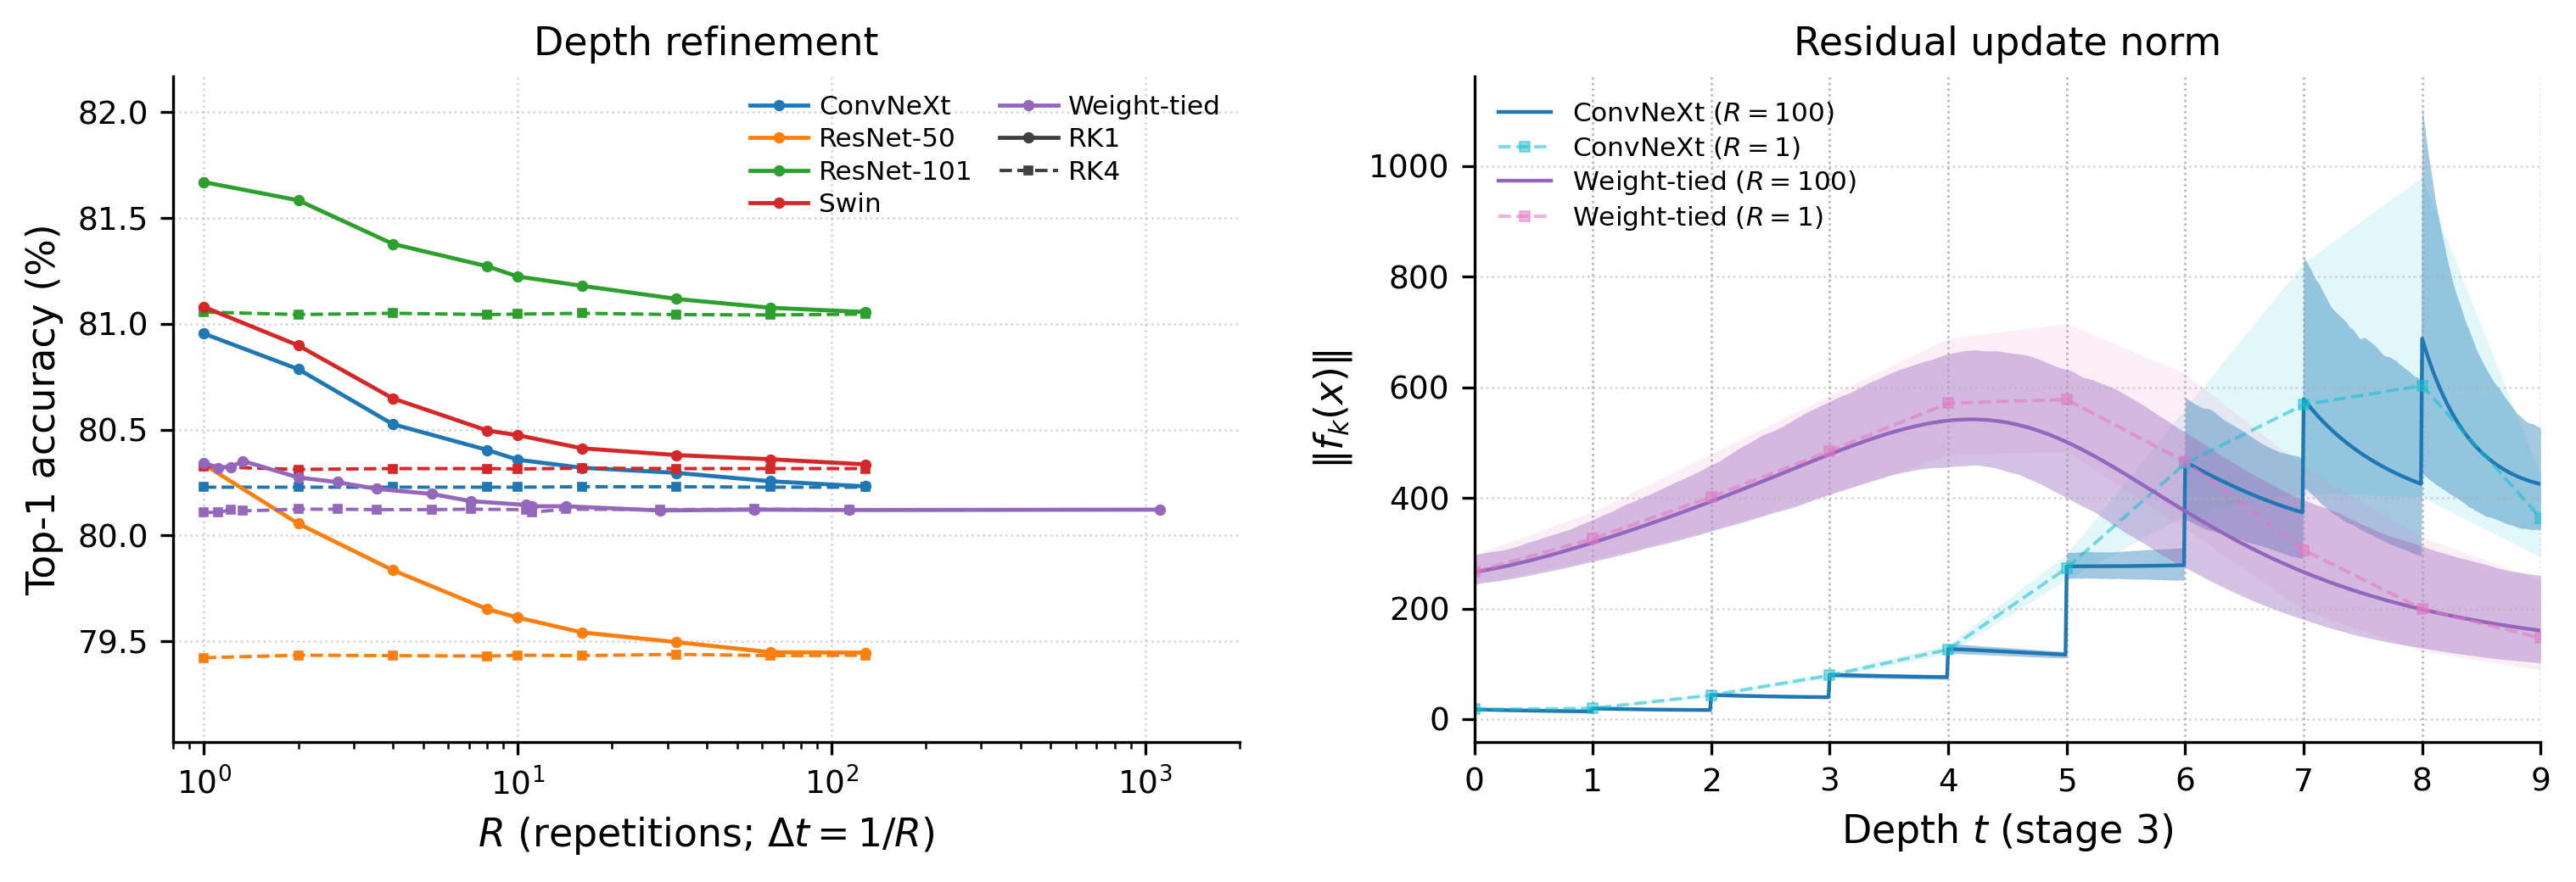
\includegraphics[width=\textwidth]{figures/teaser.png}
    \caption{\textbf{Left:} top-1 vs.\ repetitions $R$ (solid: Euler / RK1; dashed: RK4),
    with $\Delta t{=}1/R$ so $T{=}n$ is conserved
    (weight-tied: $nR$ applications of the shared block).
    \textbf{Right:} residual-field norm $\|f(x)\|$ along stage~3
    (mean and P5--P95 over 500 images). ConvNeXt is piecewise constant in depth;
    the weight-tied model is a single smooth autonomous field.
    See \cref{sec:teaser-b}.}
    \label{fig:teaser}
\end{figure*}

\Cref{sec:weight_tied} showed that one shared block nearly matches a standard
ConvNeXt stage~3 (independent per-block weights).
We now test whether residual blocks behave as one-step Euler updates of a vector field:
if so, repeating each update $R$ times with step $\Delta t{=}1/R$---without
fine-tuning---should preserve the trained horizon $T{=}n$ and the function the network
computes.
Convergence of the refinement by itself is not diagnostic, since any residual block
with Lipschitz $f$ has a continuous limit (\cref{app:random-init}); the informative
quantities are what the limit retains and how far the native path is from it.
We apply this probe to weight-tied and standard networks; the geometry of the
resulting trajectories is deferred to \cref{sec:geometrical_analysis}.

A residual block computes $x + f(x)$~\citep{he2016resnet}.
With step size $1$, that is exactly one step of the explicit Euler method for the ODE
$\dot x = f(x,t)$~\citep{e2017proposal,haber2017stable,lu2018beyond}.
Write the residual of block $i$ as
\begin{equation}
    f_i(x) \;=\; \mathrm{block}_i(x) - x.
    \label{eq:residual}
\end{equation}
Then the native network is one Euler step of size $1$ per block. Over a stage of $n$ blocks
(e.g.\ $n{=}9$ in ConvNeXt-T stage~3), starting from the output $x_0$ of the previous stage,
\begin{equation}
    x_{i+1} \;=\; x_i + f_i(x_i),
    \qquad
    x_n \;=\; x_0 + \sum_{i=0}^{n-1} f_i(x_i).
    \label{eq:euler-stage}
\end{equation}

Some argue that this algebraic form is already enough to call the network an Euler
solver~\citep{e2017proposal,haber2017stable,lu2018beyond},
but algebraic form alone is not sufficient evidence:
\citet{queiruga2020continuousindepthneuralnetworks} argue that ResNets fail to be meaningful
dynamical integrators beyond that syntactic similarity, and
\citet{sander2022residualneuralnetworksdiscretize} show that a ResNet approaches its associated
Neural ODE only when the residual maps vary smoothly in depth
(otherwise the discrete stack need not be a consistent discretization of a single continuous flow).

We suggest reading the stage as a \emph{sum of several ODEs}, one per block, where the network
is trained to solve each unit interval with a single Euler step.
The continuous object behind~\eqref{eq:euler-stage} is therefore
\begin{equation}
    x_n \;=\; x_0 + \sum_{i=0}^{n-1} \int_{i}^{i+1} f_i\bigl(x(t)\bigr)\,dt,
    \label{eq:sum-of-integrals}
\end{equation}
or, block by block,
\begin{equation}
    x_{i+1} \;=\; x_i + \int_{i}^{i+1} f_i\bigl(x(t)\bigr)\,dt.
    \label{eq:block-integral}
\end{equation}
Here the sum is the stack of residual blocks, and each integral is the continuous counterpart of
the one-step update in~\eqref{eq:euler-stage}: instead of taking one Euler step of size $1$,
we integrate $f_i$ over the unit interval $[i,i+1]$, keeping the horizon of each block equal to $1$.
For a stage with $n$ blocks trained at unit step, the stage horizon is therefore
\begin{equation}
    T \;=\; n
    \qquad\text{(ConvNeXt-T stage~3: $n{=}9$, so $T{=}9$).}
    \label{eq:horizon-T}
\end{equation}

\paragraph{Repetitions $R$.}
Throughout the paper we use a single refinement parameter $R$ (\emph{repetitions}).
For a non-tied stage, $R{=}2$ means each of the $n$ blocks is applied twice, for $nR$ residual
updates in total.
For a weight-tied stage, $R{=}2$ means the \emph{same} shared block is applied $nR{=}18$ times.
In both cases we set the Euler step from the trained horizon,
\begin{equation}
    \Delta t \;=\; \frac{1}{R}
    \qquad\Rightarrow\qquad
    T \;=\; nR\cdot\Delta t \;=\; n,
    \label{eq:delta-from-R}
\end{equation}
so refining never changes the integration time---only the resolution.

\textbf{Plain} interpolation keeps the field piecewise constant on each block and discretizes
the integral with $R$ Euler sub-steps of size $\Delta t = 1/R$:
\begin{equation}
    \int_{i}^{i+1} f_i\bigl(x(t)\bigr)\,dt
    \;\approx\;
    \sum_{r=0}^{R-1} \Delta t\, f_i\bigl(x_{i + r\Delta t}\bigr).
    \label{eq:plain-euler}
\end{equation}
Equivalently, over the whole stage the refined trajectory is
\begin{equation}
    x_T \;=\; x_0 + \sum_{i=0}^{T-1} \sum_{r=0}^{R-1} \Delta t\, f_i\bigl(x_{i + r\Delta t}\bigr),
    \qquad \Delta t = \tfrac{1}{R}.
    \label{eq:refined-stage}
\end{equation}
When $R{=}1$,~\eqref{eq:refined-stage} recovers the original network~\eqref{eq:euler-stage}.
As $R$ grows with $T{=}n$ fixed, the scheme approaches the continuous
limit~\eqref{eq:sum-of-integrals}; we also compare against Midpoint (RK2) and RK4 on the same horizon.

In a weight-tied stage the residual field is the same at every depth,
$f_i \equiv f$ for all $i$. Then~\eqref{eq:sum-of-integrals} collapses to a single
autonomous integral over $[0,T]$ with $T{=}n$:
\begin{equation}
    x_T \;=\; x_0 + \int_{0}^{T} f\bigl(x(t)\bigr)\,dt.
    \label{eq:weight-tied-ode}
\end{equation}
Inference uses $nR$ applications of $f$ with $\Delta t{=}1/R$; training uses $R{=}1$
($n$ steps of size $1$), hence $T{=}9$ for our shared ConvNeXt-T.


\subsubsection{Ablations}
\label{sec:looping-ablations}

We apply the refinement~\eqref{eq:refined-stage} (plain interpolation, $T$ conserved via
$\Delta t{=}1/R$) to our ConvNeXt-T, our weight-tied ConvNeXt-T, Swin-T, ResNet-50 and
ResNet-101 (ImageNet-1k validation, top-1).
\Cref{fig:teaser} (left) summarises the sweep over $R$; numbers are in
\cref{tab:r-ablation}.

Accuracy decreases monotonically as $R$ grows and plateaus at a continuous limit that
matches RK4.
Euler (RK1), Midpoint (RK2) and RK4 all converge to the \emph{same} accuracy once the
step is fine enough; full Mid/RK4 tables are in \cref{app:solvers}.
(Matched top-1 alone does not prove a shared state $x_T$; we check endpoint agreement
of the solvers later in \cref{app:solver-endpoints}.)
The trained network itself (Euler, $R{=}1$) is \emph{not} at that limit; it is the best
point of every sweep.
Keeping the nine steps of size $\Delta t{=}1$ but swapping Euler for RK4 already lands on
the limit, both in accuracy and in the stage-3 state (\cref{app:solver-endpoints}), and
costs $0.6$--$0.9$ points on the untied models ($0.2$ on the weight-tied one):
the decoder is tuned to the state produced by a single Euler step of size~$1$, not to
the flow it approximates.

\begin{table}[t]
    \centering
    \caption{Plain Euler refinement with $\Delta t{=}1/R$ ($T$ conserved). Top-1 (\%).
    For weight-tied, $R$ means $9R$ applications of the shared block
    (exact $9R$ when available; else nearest measured depth$^\ast$).
    ODE limit: RK4 at the finest step in each sweep.}
    \label{tab:r-ablation}
    \small
    \setlength{\tabcolsep}{2.8pt}
    \begin{tabular}{lrrrrr}
        \toprule
        $R$ ($\Delta t$) & CNX-T & Swin-T & R-50 & R-101 & Tied \\
        \midrule
        $1$ ($1$)       & 80.95 & 81.08 & 80.34 & 81.67 & 80.34 \\
        $2$ ($0.5$)     & 80.79 & 80.90 & 80.06 & 81.58 & 80.27 \\
        $4$ ($0.25$)    & 80.53 & 80.65 & 79.84 & 81.38 & 80.22$^\ast$ \\
        $10$ ($0.1$)    & 80.36 & 80.47 & 79.61 & 81.22 & 80.14$^\ast$ \\
        $32$ ($0.03$)   & 80.30 & 80.38 & 79.50 & 81.12 & 80.14$^\ast$ \\
        $128$ ($0.008$) & 80.23 & 80.34 & 79.45 & 81.06 & 80.12$^\ast$ \\
        \midrule
        ODE limit       & 80.23 & 80.32 & 79.43 & 81.05 & 80.12 \\
        Gap ($R{=}1\!\to$ODE) & $-0.72$ & $-0.76$ & $-0.91$ & $-0.62$ & $-0.22$ \\
        \bottomrule
    \end{tabular}
    \vspace{2pt}
    {\footnotesize $^\ast$Nearest measured shared depth at $T{=}9$:
    32, 96, 128, 1024 steps respectively (exact $9R$ would be 36, 90, 288, 1152).}
\end{table}

\paragraph{Wrong step size.}
Repeating blocks without shrinking the step (e.g.\ $R{=}10$ with $\Delta t{=}1$, so
$T$ grows tenfold) collapses every pretrained model to chance
($\approx 0.1\%$--$1\%$ top-1).
The same holds for the weight-tied network when $T$ leaves the trained horizon
(\cref{fig:horizon,fig:shared-fractional}).
The Euler step must be $\Delta t{=}1/R$, equivalently $T{=}n$ for an $n$-block stage
($T{=}9$ when $n{=}9$).
The trajectory dynamics behind this collapse are analysed in \cref{sec:beyond_horizon}.

\paragraph{Weight-tied fractional $R<1$.}
\Cref{fig:shared-fractional} reports the shared network at fixed $T{=}9$ with fewer
than nine steps ($R<1$, i.e.\ $9R$ applications with $\Delta t{=}1/R>1$); the numbers,
including Midpoint, are in \cref{tab:app-shared-t9}.
Large steps need a higher-order solver: at $R{=}4/9$ (4 steps), RK4 reaches $78.9\%$ while
Euler falls to $67.8\%$; Euler with $R{=}2/9$ ($\Delta t{=}4.5$) is unstable ($5.9\%$).
For $R\geq 7/9$, all three solvers sit within $0.3$ points of the trained baseline.

\begin{figure}[t]
    \centering
    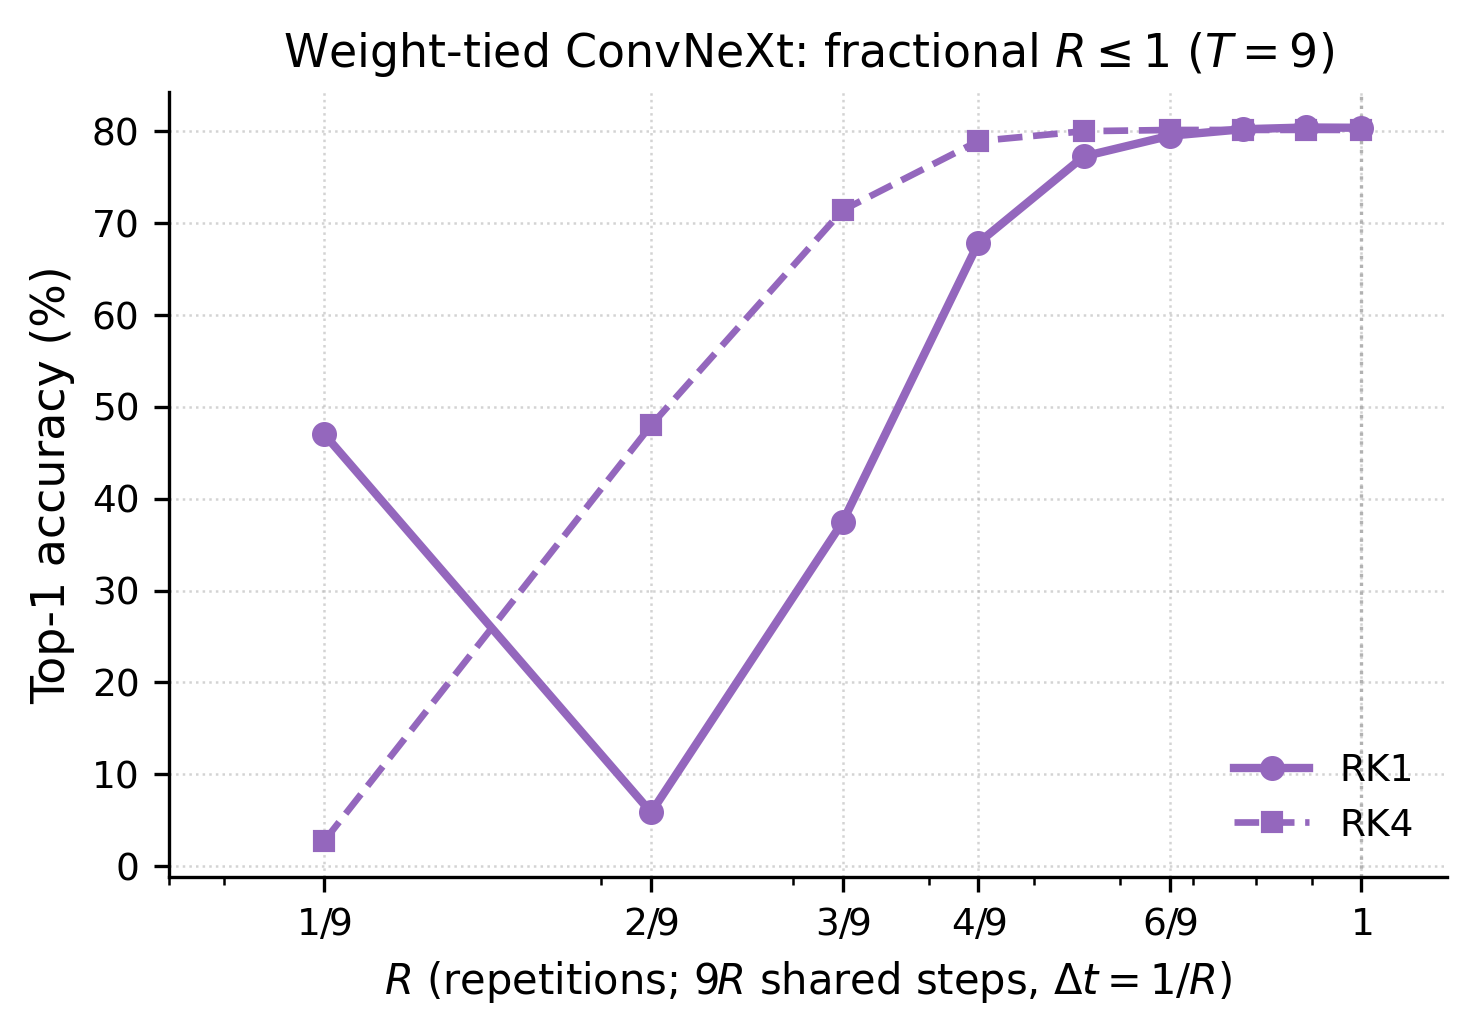
\includegraphics[width=\linewidth]{figures/shared_fractional.png}
    \caption{Shared ConvNeXt-T at fixed $T{=}9$ for fractional $R\leq 1$
    (RK1 solid, RK4 dashed).}
    \label{fig:shared-fractional}
\end{figure}

\paragraph{Horizon, not resolution.}
Varying the number of unit steps at $\Delta t{=}1$ (so $T$ grows) or varying $\Delta t$ at
fixed $R{=}1$ (9 steps; $T{=}9\cdot\Delta t$) both peak at $T{=}9$
(\cref{fig:horizon}): the classification head expects the state reached after that
integration time.
Integrating too short or too long degrades smoothly near $T{=}9$ and collapses far from it.
We conclude that the best Euler step is the one that preserves the trained horizon:
$\Delta t{=}1/R$ for every model (non-tied and weight-tied).

\begin{figure}[t]
    \centering
    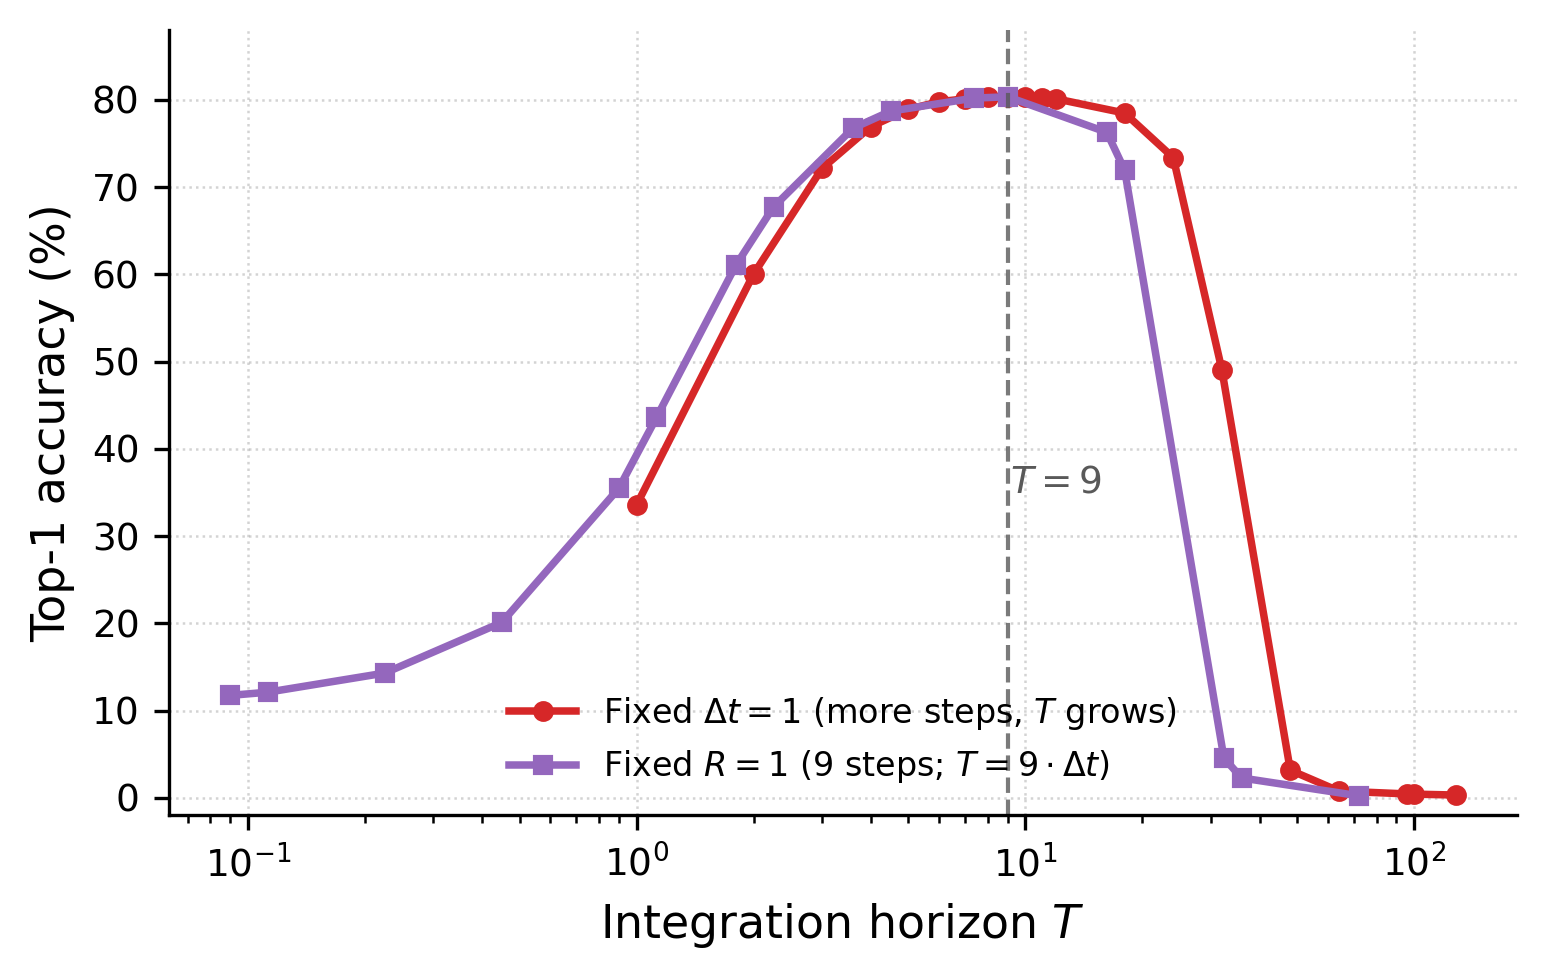
\includegraphics[width=\linewidth]{figures/horizon_ablation.png}
    \caption{Shared ConvNeXt-T: top-1 vs.\ horizon $T$.
    Red: fixed $\Delta t{=}1$, more steps ($T$ grows).
    Purple: fixed $R{=}1$ (9 steps), varying $\Delta t$ ($T{=}9\cdot\Delta t$).
    Both peak at the trained horizon $T{=}9$.}
    \label{fig:horizon}
\end{figure}

\paragraph{Do refined blocks land on the same $x$?}
Near-baseline accuracy does \emph{not} mean that $R$ Euler steps of size $1/R$
reproduce the unit-step state.
\Cref{fig:dist-r1} compares the refined ConvNeXt-T trajectory ($R{=}100$,
$\Delta t{=}0.01$) with the native $R{=}1$ trajectory on the same images, in $\ell_2$
distance (top, next to both state norms) and cosine similarity (bottom)
(massive channel removed from the metrics, see \cref{sec:massive_activations};
$N{=}500$ images).
Three facts stand out.
\begin{itemize}
    \item \textbf{Within each block} the refined trajectory moves \emph{toward} the
    parallel $R{=}1$ checkpoint: the distance decays and the cosine rises until the
    block ends, so the refinement is not drifting away from the one-step endpoint of
    that block.
    \item \textbf{Across blocks} the gap grows: the block-end distance rises from
    $\approx 5.6$ to $\approx 76$ at $t{=}9$, against $\|x\|\approx 203$ at the stage exit,
    i.e.\ a relative gap $\|x^{(R)}-x_{R{=}1}\|/\|x\|\approx 0.36$.
    \item \textbf{The gap is a rotation.} The block-end cosine drops from $0.99$ to $0.93$
    ($\sim\!21^\circ$), while $\|x\|$ differs by only $\approx 3\%$ ($203$ vs.\ $210$);
    a pure rescaling of that size would account for a distance of $\approx 7$, not $76$.
\end{itemize}
Each block therefore implements a \emph{different} map than its one-step counterpart
once the input has already drifted; local refinement stays contractive toward the
current block's $R{=}1$ target, but errors accumulate through the switched stack and
the final $x_T$ points in a different direction from the native one.

\begin{figure}[t]
    \centering
    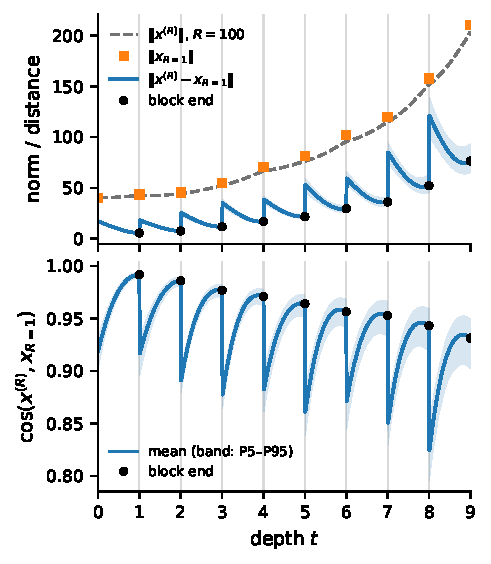
\includegraphics[width=\linewidth]{figures/dist_cos_r1.pdf}
    \caption{ConvNeXt-T, $R{=}100$, $\Delta t{=}0.01$, against the native $R{=}1$ path.
    \textbf{Top:} $\|x^{(R)}(t)-x_{R{=}1}\|$ (solid), with the state norms of both paths
    for scale (dashed: $R{=}100$; squares: $R{=}1$).
    \textbf{Bottom:} $\cos(x^{(R)},x_{R{=}1})$.
    Mean and P5--P95 over 500 images; massive channel ignored; dots mark block ends.
    The norms nearly coincide while the block-end gap grows with depth: the mismatch is
    mostly in angle.}
    \label{fig:dist-r1}
\end{figure}

\paragraph{Finetuning stage~4 and the head after unrolling.}
As a complementary check, we freeze stem and stages~1--3 and finetune only stage~4
and the classification head on the unrolled transport (horizon $T{=}9$ conserved).
On ConvNeXt-T with $R{=}3$ ($\Delta t{=}1/3$) this recovers $80.93\%$ top-1---within
$0.04$ points of the untied baseline ($80.97\%$).\footnote{Script:
\texttt{scripts/finetune\_s4\_r\_convnext.py}.
For contrast, $R{=}3$ with $\Delta t{=}1$ (broken horizon $T{=}27$) collapses to
$41\%$ \emph{without} finetuning (\texttt{convnext\_r3\_quick}).}
% TODO: sync Leonardo run directories for the numbers below.
The same protocol at the fine step used in \cref{fig:dist-r1} yields
$\mathrm{XX}\%$ top-1 for ConvNeXt-T at $R{=}100$ ($\Delta t{=}0.01$)
and $\mathrm{XX}\%$ for the weight-tied model at $R{=}100$ ($900$ shared steps, $\Delta t{=}0.01$)
after $10$ epochs at learning rate $10^{-6}$
(\texttt{finetune\_s4\_r100\_convnext.sh}, \texttt{finetune\_s4\_d900\_shared\_convnext.sh}).
So even though the refined stage-3 endpoint differs substantially from the native
$x_T$ in representation space, a light adaptation of the decoder largely restores
accuracy when $T$ is kept: the transport changes; the head can re-read it.

\paragraph{Takeaway.}
Three facts summarise the looping probe.
\emph{(i)~Discretisation.}
Refining the Euler step at fixed~$T$ does \emph{not} reproduce the native one-step
state: at $R{=}100$, after removing the massive channel, the stage-3 endpoint has
relative $\ell_2$ gap $\approx 0.36$ to the parallel $R{=}1$ path
(\cref{fig:dist-r1}) and cosine $\approx 0.93$ ($\sim\!21^\circ$), so the mismatch is
mostly angular rather than a pure rescaling of $\|x\|$.
The weight-tied stage does not accumulate this error: its cosine to the $R{=}1$ path
settles at $\approx 0.98$ (relative gap $\approx 0.20$) instead of falling block after
block (\cref{sec:refinement_error}).
\emph{(ii)~Continuous limit.}
That gap is \emph{not} solver noise: Euler and RK4 at the same fine step, and Euler
$R{=}100$ vs.\ $R{=}200$, agree on $x_T$ to relative distance $\ll 10^{-2}$
(\cref{app:solver-endpoints}).
A continuous limit of the piecewise residual field therefore exists, but it is not
the trained $R{=}1$ discretisation.
Neither fact is specific to training.
A random-initialisation control (\cref{app:random-init}) shows that the blocks of all
five architectures, random or trained, converge to a single $\hat x_T$ under refinement.
How far the one-step path lies from that limit is governed mainly by how far each block
moves the state, $\|f_i(x_i)\|/\|x_i\|$: weights trained to be used once produce steps of
$30$--$90\%$ of $\|x\|$ and sit $10$--$21^\circ$ from their limit, too far for one Euler step
to track the flow.
At the same relative step, training moves that distance in an architecture-dependent
direction: trained Swin-T and ConvNeXt-T are closer to their limit than a random field
($19.5^\circ$ vs.\ $47.6^\circ$, $21.1^\circ$ vs.\ $30.2^\circ$), the weight-tied model is level
with it ($10.9^\circ$ vs.\ $11.9^\circ$), and the ResNets are farther.
What distinguishes the trained networks is therefore not \emph{whether} the refinement
converges but \emph{how} the trajectory is built: one shared block applied throughout
the stage versus nine different blocks applied once each.
\Cref{sec:geometrical_analysis} contrasts the two regimes.
\emph{(iii)~Accuracy.}
Top-1 nevertheless barely moves under refinement without training, because the head
cares about class margins, not isometry of the full feature space.
Finetuning stage~4 and the head recovers $80.93\%$ at $R{=}3$ and
$\mathrm{XX}\%$ / $\mathrm{XX}\%$ for ConvNeXt-T / weight-tied at $R{=}100$
% TODO: fill XX from Leonardo S4+head runs (10 epochs, lr=1e-6).
---essentially the baseline once the decoder adapts.
In short: residual blocks admit a well-defined fine-step flow, as any Lipschitz residual
field does; their single unit step is too large to be a consistent solver of that flow;
the flow nonetheless retains the network's function (the limit keeps $\approx 80\%$ top-1,
which a random field cannot show), accuracy survives because the head is tolerant, and a
light S4+head adaptation closes almost all of the remaining gap.

Influenced by continuous-in-depth models~\citep{queiruga2020continuousindepthneuralnetworks,chang2018multilevel},
we also tried replacing the piecewise-constant schedule
$\theta_t=\theta_{\lfloor t\rfloor}$ by a bilinear blend of consecutive block weights.
It performs relatively badly on every architecture (e.g.\ $-6.6$ points on ConvNeXt-T at
$R{=}128$ vs.\ plain); full numbers and the residual-norm trajectories are in
\cref{app:bilinear}.

\subsubsection{Piecewise vs.\ smooth residual fields}
\label{sec:teaser-b}

\Cref{fig:teaser}~(right) makes the dynamical difference between the two regimes concrete.
In the non-tied ConvNeXt, $\|f_k(x)\|$ is approximately constant inside each block and
jumps at integer depths: a \emph{smooth function by parts}, i.e.\ an autonomous field on
each unit interval $[i,i+1]$ with discontinuous switches of $\theta$ between blocks
(\cref{eq:sum-of-integrals}).
In the weight-tied model the same shared $f$ is applied for the whole stage, so the
residual norm evolves as one continuous curve that rises and then decays
(\cref{eq:weight-tied-ode}).
Markers at $R{=}1$ sit on those curves; refining to $R{=}100$ fills in the
intra-block path without changing its global shape.
This is the geometric counterpart of the accuracy tables: refining a switched stack
converges to a slightly worse continuous limit, while refining a shared field stays near
the trained accuracy as long as $T$ is held fixed.
\Cref{sec:geometrical_analysis,sec:overparametrized_undoing} analyse these trajectories
in more detail---in particular, how untied blocks redirect the state between integer
depths even though each intra-block piece remains integrable.

\subsection{Geometrical analysis of feature trajectories}
\label{sec:geometrical_analysis}

In this section we analyze the geometry of the trajectories regarding the weight-tied convnext vs the standard convnext.
We also compare the standard convnext with resnet and swin, whose properties are very similar since they are non weight-tied and
the network learned to make the blocks perform an unique functionality of one step, so there is no reason for the network to learn a more
complex dynamic.

\subsubsection{Massive activations excluded from analysis}
\label{sec:massive_activations}

After analyzing some trajectories on our first aproach, they seemed too homogeneos in convnext and swin cases, so we analyzed the features and
founded the so called massive activations \cite{sun2024massiveactivationslargelanguage}. In convnext shared and non-shared there is one channel that grows indifinetly.
We did a similar analysis and concluded the same as \cite{sun2024massiveactivationslargelanguage}

\subsubsection{Trajectories of weight-tied convnxt vs standard convnext}


\subsubsection{Trajectory analysis of weight-tied convnext}
\label{sec:refinement_error}
Inpired by some of the metrics of \cite{pandey2026trajectorygeometrytransformerrepresentations} we perform an analysis of the trajectories
ignoring the massive channels of Convnext and the massive tokens of swin. Resnet does not show signs of massive activations.

In weight-tied convnext we can see in Figure \ref{fig:teaser} right the norm of the velocity, that is $f(x(t))$ that has a shape of a bell curve.
This information only shows if the point is moving or not, but it doesn't tell if it rotates or move towards the same direction.
That's why we plot several new metrics:

\textbf{Acceleration}

Here we decompose the acceleration vector into the sum of two components: The tangential and normal accelerations with respect to the velocity.
Note, that in a high-dimentional space of 300,000 dimensions (the case of Stage 3 in convnext), there are 299.999 dimentions that are normal with the velocity, and only 1 that is tangent.
The tangent component can be negative or positive with respect to the velocity that is, it reduces or increases the current velocity in this 1D line, but we cna only analyze the norm of the normal acceleration.
Even in a such space, that tangential acceleration has a big representation.

We can see

\textbf{Angular acceleration}
\textbf{Trajectory curvature}

\textbf{The shape of the trajectory}

With all this tools, we conclude that the trajectory at the start rotates at high speeds, giving the trajectory a high curvature,
but with low velocity norm, that implies that it does small steps changing constantly of direction. The model is computing the direction where it has to accelerate the point to.

After that, the model starts to accelerate towards one direction, angular speed decreases, norm of angular acceleration increases due to the reduction of velocity
the result is a major reduction on the curvature of the trajectory, while tangential acceleration hits its maximum. The model is expanding the most important features.

Finally, angular acceleration decreases, tangential acceleration rapidly decreases, becoming negative, the velocity decreases, the angular velocity increases again, and curvature raises again. We have the same
scenario as in the first phase. The model is refining features again.

We observe that for the 500 images we analyzed, the trajectory is mostly of this form. But in the variance analysis,
the velocity has its maximum variance on the second phase since the model is pushing the features of different classes apart from the origin in different directions.

\subsubsection{Refinement error: accumulated vs.\ bounded}
\label{sec:refinement_error}

\begin{figure*}[t]
    \centering
    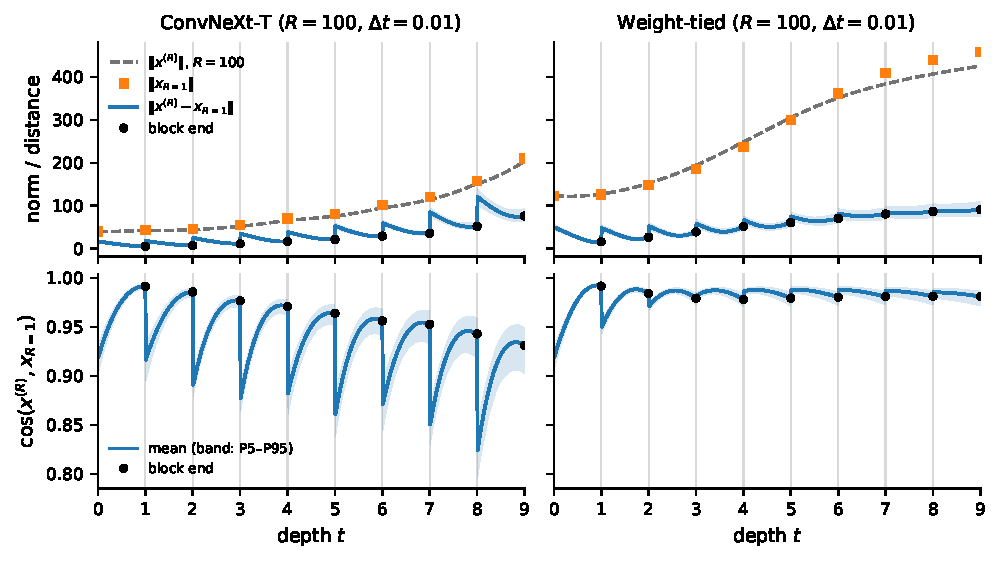
\includegraphics[width=\textwidth]{figures/dist_cos_r1_compare.pdf}
    \caption{Refined vs.\ native ($R{=}1$) stage-3 path for the standard (left) and
    weight-tied (right) ConvNeXt-T.
    \textbf{Top:} $\|x^{(R)}-x_{R{=}1}\|$ (solid) with both state norms for scale
    (dashed: refined; squares: native).
    \textbf{Bottom:} $\cos(x^{(R)},x_{R{=}1})$.
    Mean and P5--P95 over the same 500 images; massive channel ignored; dots mark the end
    of each native step.
    The switched stack accumulates angle at every block; the shared field saturates.}
    \label{fig:dist-r1-compare}
\end{figure*}

\Cref{fig:dist-r1-compare} repeats the comparison of \cref{fig:dist-r1} for the
weight-tied network.
Both models start the same way: after the first native step the cosine to the $R{=}1$
path is $0.99$.
They then diverge.
In the standard ConvNeXt-T the block-end cosine keeps falling, to $0.93$ at $t{=}9$:
each block receives an input that has already drifted and adds its own discretisation
error on top.
In the weight-tied model it settles at $\approx 0.98$ after two or three steps and stays
there for the rest of the stage, so a single autonomous field keeps the refinement error
bounded instead of accumulating it.
The norms also behave differently: in ConvNeXt-T they nearly coincide ($203$ vs.\ $210$),
whereas the weight-tied refined path ends about $7\%$ shorter ($427$ vs.\ $458$), so part
of its smaller gap is radial.
% TODO: relate the bounded error to the contractivity of the shared field.

\subsubsection{Integrating beyond the trained horizon}
\label{sec:beyond_horizon}
% TODO: constant velocity regime: f(x) saturates, x grows along a fixed direction for T >> n.
There is big difference between weight-tied convnext and standard convnext: First one reaches a velocity plateau
where the input just grows indifinetly in the same direction.

In standard convnext, swin and resnet are different, we used R=100 with euler step 1,
since the blocks use different parameters and the network was not trained to reuse params,
it has a similar dynamics as the R=100 with Euler step of 0.01 but with more magnitude.

\subsection{Are over-parametrized networks undoing what the previous layers have done?}
\label{sec:overparametrized_undoing}

\Cref{sec:weight_tied} showed that one shared stage-3 block nearly matches nine
independent ones ($-0.61$ top-1 points, $33\%$ fewer parameters).
A natural explanation is that the untied stack is over-parametrised along depth:
consecutive blocks need not push the state in a coherent direction, and part of
what block $k{+}1$ does can cancel what block $k$ just did.
We test that claim directly on feature trajectories, using the same 500 ImageNet
validation images (one per class) as in \cref{sec:geometrical_analysis}, stage~3
only, with the massive channel removed (\cref{sec:massive_activations}).

\paragraph{Setup.}
For each image we integrate the stage from $t{=}0$ to $t{=}9$ at native resolution
($R{=}1$) and under Euler refinement ($R{=}100$, $\Delta t{=}0.01$), and reduce every
spatial feature coordinate whose net displacement $|\Delta_i|=|x_i(9)-x_i(0)|$ is above
the per-image median.
We partition the trajectory into the nine unit intervals $[k,k{+}1]$ (native blocks
in ConvNeXt-T; the same time bins in the weight-tied model) and write
$\mathrm{d}x_k$ for the displacement of a coordinate over interval $k$.
The scalars we report are means $\pm$ std over the 500 images
(\cref{tab:undo}):
\begin{itemize}
    \item \emph{straightness}: $\|\sum_k\mathrm{d}x_k\|\,/\,\sum_k\|\mathrm{d}x_k\|$
    in feature space (path length vs.\ net displacement);
    \item \emph{wasted motion}: $1-\sum_i|\mathrm{net}_i|/\sum_{k,i}|\mathrm{d}x_{k,i}|$,
    the fraction of per-coordinate travel that cancels before $t{=}9$;
    \item $\cos(\mathrm{d}x_k,\mathrm{d}x_{k+1})$: mean cosine between consecutive
    block displacements;
    \item \emph{undo fraction}: when $\mathrm{sign}(\mathrm{d}x_k)$ flips at the next
    block, the cancelled mass
    $\min(|\mathrm{d}x_k|,|\mathrm{d}x_{k+1}|)$ normalised by $\sum|\mathrm{d}x_k|$;
    \item \emph{zig-zag share}: mass-weighted share of coordinates that reverse at
    least twice across the nine blocks;
    \item \emph{sign flips at $t\in\mathbb{N}$}: fraction of consecutive steps whose
    sign changes exactly at integer depths (block boundaries).
\end{itemize}

\begin{table*}[t]
    \centering
    \caption{Pooled stage-3 trajectory statistics over 500 ImageNet images
    (massive channel ignored; coordinates with $|\Delta_i|$ above the per-image median).
    Weight-tied vs.\ standard ConvNeXt-T at native ($R{=}1$) and refined ($R{=}100$)
    resolution. Mean $\pm$ std across images.}
    \label{tab:undo}
    \scriptsize
    \setlength{\tabcolsep}{3.5pt}
    \resizebox{\textwidth}{!}{%
    \begin{tabular}{llccccccccc}
\toprule
Model & $R$ & straightness & wasted motion & monotone share & $\cos(\Delta x_k,\Delta x_{k+1})$ & reversal rate & undo fraction & zig-zag share & sign flips at $t\in\mathbb{N}$ & median $t_{50}$ \\
\midrule
Weight-tied ConvNeXt & 100 & 0.78$\pm$0.02 & 0.19$\pm$0.01 & 0.73$\pm$0.02 & 0.92$\pm$0.01 & 0.11$\pm$0.01 & 0.02$\pm$0.00 & 0.14$\pm$0.02 & 0.00$\pm$0.00 & 4.09$\pm$0.16 \\
ConvNeXt-T & 100 & 0.50$\pm$0.01 & 0.48$\pm$0.01 & 0.21$\pm$0.01 & 0.17$\pm$0.01 & 0.45$\pm$0.00 & 0.25$\pm$0.00 & 0.90$\pm$0.00 & 0.45$\pm$0.00 & 7.21$\pm$0.15 \\
Weight-tied ConvNeXt & 1 & 0.72$\pm$0.02 & 0.25$\pm$0.02 & 0.63$\pm$0.03 & 0.77$\pm$0.03 & 0.18$\pm$0.01 & 0.05$\pm$0.01 & 0.34$\pm$0.03 & 0.18$\pm$0.01 & 5.00$\pm$0.09 \\
ConvNeXt-T & 1 & 0.50$\pm$0.01 & 0.48$\pm$0.01 & 0.22$\pm$0.01 & 0.16$\pm$0.01 & 0.45$\pm$0.00 & 0.25$\pm$0.00 & 0.90$\pm$0.00 & 0.45$\pm$0.00 & 7.82$\pm$0.38 \\
\bottomrule
\end{tabular}

    }
\end{table*}

\begin{figure*}[t]
    \centering
    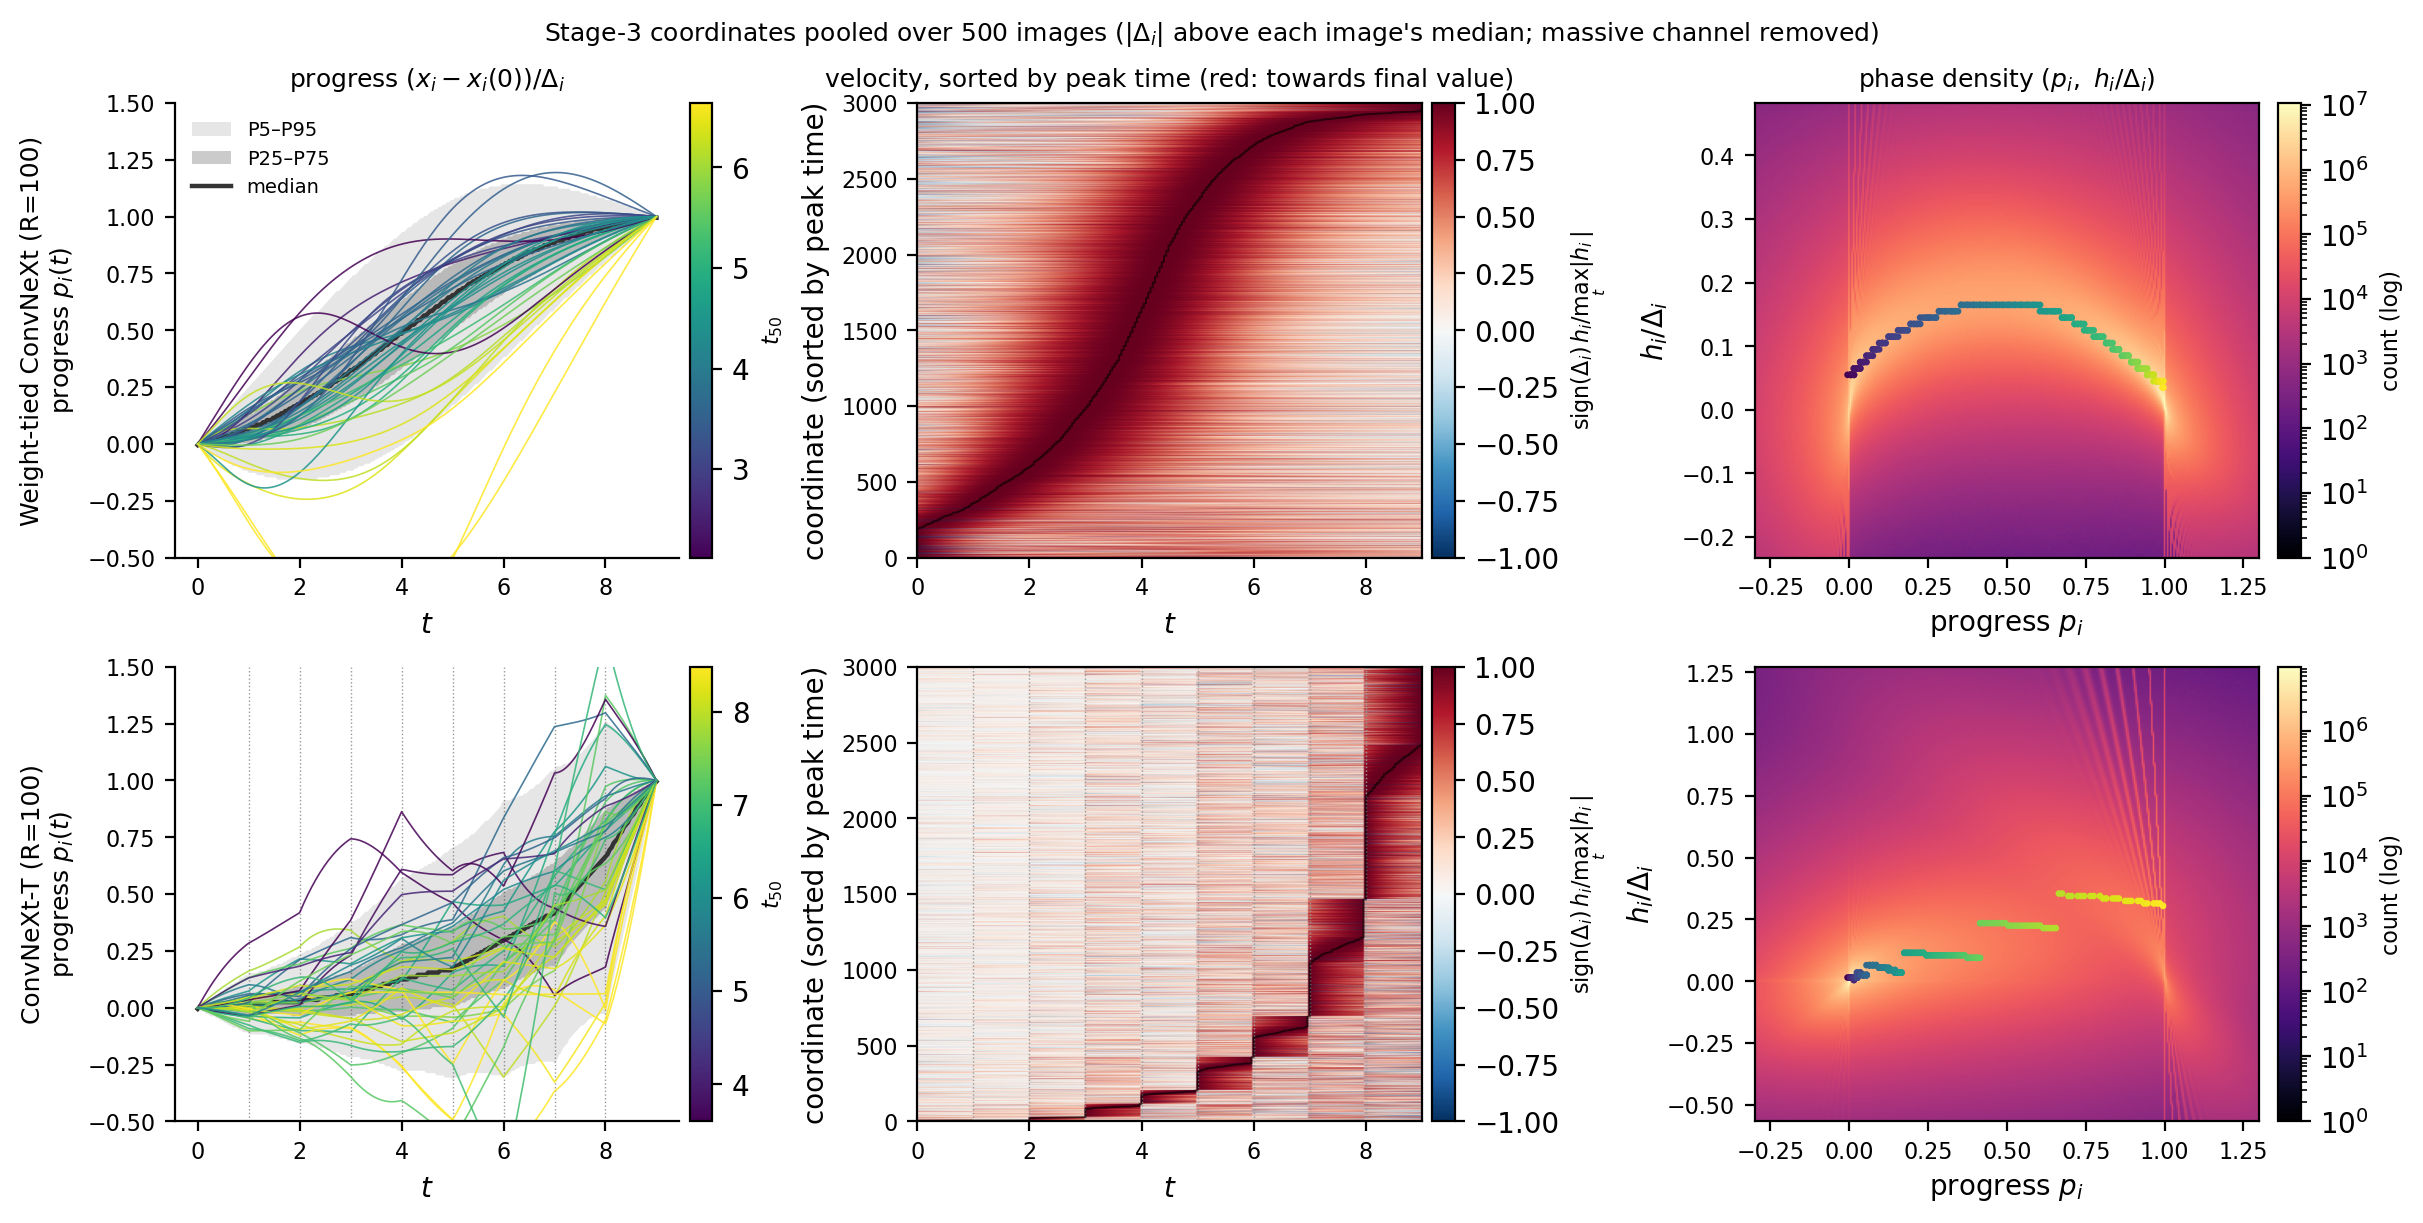
\includegraphics[width=\textwidth]{figures/pooled_dynamics.png}
    \caption{Stage-3 coordinates pooled over 500 images ($R{=}100$; massive channel
    removed; $|\Delta_i|$ above the per-image median).
    \textbf{Top:} weight-tied ConvNeXt; \textbf{bottom:} ConvNeXt-T.
    \textbf{Left:} progress $p_i(t)=(x_i(t)-x_i(0))/\Delta_i$ (median and P5--P95;
    thin lines: random coordinates).
    \textbf{Middle:} velocity toward the final value, coordinates sorted by peak time
    (red: toward the end state; blue: away).
    \textbf{Right:} phase density $(p_i,\,h_i/\Delta_i)$.
    The shared field advances mostly monotonically; the switched stack reverses and
    rewrites features between blocks.}
    \label{fig:pooled-dynamics}
\end{figure*}

\paragraph{Results.}
\Cref{tab:undo} and \cref{fig:pooled-dynamics} give a consistent picture.
Under refinement ($R{=}100$), the weight-tied model is nearly monotone along depth:
straightness $0.78$, wasted motion $0.19$, consecutive-block cosine $0.92$, undo
fraction $0.02$, and zig-zag share $0.14$.
Sign changes at integer times are essentially absent ($0.00$).
ConvNeXt-T, with nine independent blocks, sits at the opposite extreme: straightness
$0.50$, wasted motion $0.48$ (almost half of the travel cancels), cosine $0.17$,
undo fraction $0.25$ ($\approx 12\times$ the shared value), and zig-zag share $0.90$.
Nearly half of the sign flips ($0.45$) fall exactly on block boundaries---the
discontinuities of the switched field in \cref{sec:teaser-b}, not an artefact of a
coarse step.
Native resolution ($R{=}1$) barely changes the ConvNeXt-T numbers; refining only
makes the shared field look cleaner (undo $0.05\to 0.02$), which matches the bounded
refinement error of \cref{sec:refinement_error}.

\paragraph{Functional progress along depth.}
Geometry shows wasted motion; a complementary probe asks when the stage~3 state
becomes usable by the rest of the network.
For each $k{=}1,\ldots,9$ we stop after the $k$-th residual block and classify with
the model's own trained downsample, stage~4 and head---no remaining stage~3 blocks
(\cref{fig:prefix-acc}; full ImageNet validation).
Under weight tying the top-1 rises early and smoothly: $33.6\%$ after one block,
$72.2\%$ after three, and $78.9\%$ by block~5, already close to the final
$80.3\%$.
On standard ConvNeXt-T the same frozen decoder stays weak for longer
($11.5\%$, $33.2\%$, $66.9\%$ at those depths) and only approaches the final
$81.0\%$ in the last few blocks.
Mid-stage accuracy is not a claim that early features lack information---the head
was trained on $x_T$---but it does show that the tied path enters the decoder's
operating region steadily, whereas the untied path aligns with that region late,
consistent with a transport that rewrites features before committing.

\begin{figure}[t]
    \centering
    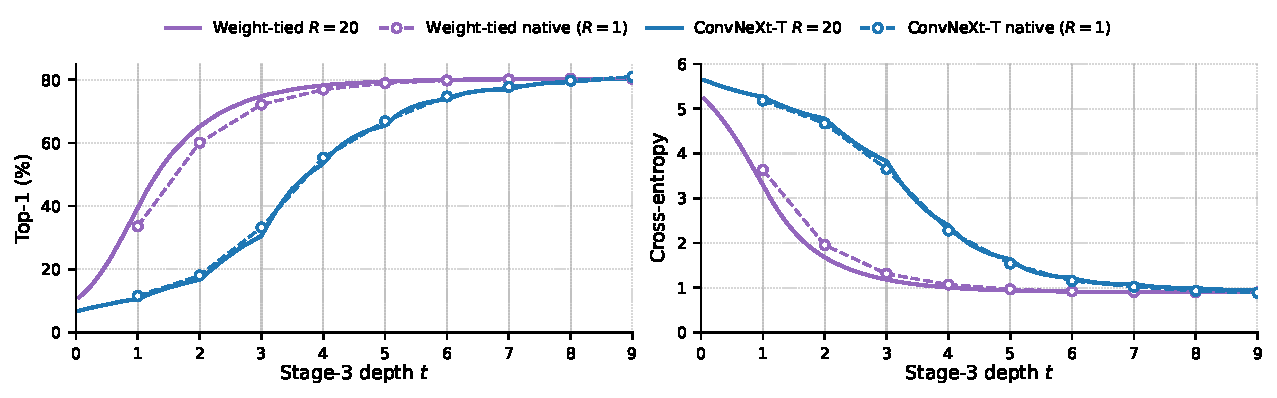
\includegraphics[width=0.7\linewidth]{figures/prefix_s4_head_acc.pdf}
    \caption{ImageNet top-1 of each model's trained stage~4+head on stage~3
    prefixes: after $k$ residual blocks, skip the rest of stage~3 and decode.
    Weight-tied features become usable earlier and more evenly; ConvNeXt-T
    concentrates most of the gain toward the end of the stage.}
    \label{fig:prefix-acc}
\end{figure}

\paragraph{Reading.}
Untied stage~3 does not implement nine steps of one transport: consecutive blocks
often point in weakly related or opposing directions and cancel a large fraction of
each other's work.
The weight-tied network cannot cancel itself in that way---a single autonomous field
has no ``next block'' with different weights---and the geometry shows almost no
undoing.
\Cref{fig:prefix-acc} makes the same contrast in function space: tied depth builds
decoder-ready features gradually, while untied depth postpones most of the usable
progress.
That is why sharing the nine blocks costs less than one top-1 point
(\cref{sec:weight_tied}): much of the untied capacity along depth is spent
rewriting features rather than accumulating a coherent displacement toward $x_T$.
The residual accuracy gap to the baseline is then more plausibly attributed to the
small, non-cancellable specialization that independent $\theta_k$ still provide, not to
a fundamentally different dynamical mechanism.

\subsection{Shared field with per-block deltas}
\label{sec:deltas}

% TODO: fine-tuning $\theta_i = \theta_{\mathrm{shared}} + \delta_i$ on top of the
% weight-tied stage-3 checkpoint; comparison to baseline and shared-only.

